% **************************************************
% Document Class Definition
% **************************************************
\documentclass[%
    paper=A4,               % paper size --> A4 is default in Germany
    twoside=true,           % onesite or twoside printing
    openright,              % doublepage cleaning ends up right side
    parskip=half,           % spacing value / method for paragraphs
    chapterprefix=true,     % prefix for chapter marks
    11pt,                   % font size
    headings=normal,        % size of headings
    bibliography=totoc,     % include bib in toc
    listof=totoc,           % include listof entries in toc
    titlepage=on,           % own page for each title page
    captions=tableabove,    % display table captions above the float env
    chapterprefix=false,    % do not display a prefix for chapters
    appendixprefix=false,   % but display a prefix for appendix chapter
    draft=false,            % value for draft version
]{scrreprt}%

\usepackage{enumitem}       % Packed itemize
%\usepackage{layouts}       % Just to print the layout of this document
                            %     Please, remove in your version!


% **************************************************
% Setup YOUR master's thesis document in this file !
% **************************************************
% !TEX root = my-thesis.tex


% **************************************************
% Files' Character Encoding
% **************************************************
%% Not necessary with luaLaTeX
% 
% \PassOptionsToPackage{utf8}{inputenc}
% \usepackage{inputenc}


% **************************************************
% Information and Commands for Reuse
% **************************************************
\newcommand{\thesisTitle}{Aprendizaje no supervisado para el estudio de redes temáticas de Twitter}
\newcommand{\thesisName}{Rodrigo S. Cortez Madrigal}
\newcommand{\thesisSubject}{Tesis de Licenciatura}
\newcommand{\thesisDate}{
2021}

\newcommand{\thesisFirstSupervisor}{Dra. Marisol Flores Garrido }
\newcommand{\thesisSecondSupervisor}{Dr. Luis Miguel García Velázquez}

\newcommand{\thesisUniversityStudies}{\protect{Licenciatura en Tecnologías para la Información en Ciencias}}
\newcommand{\thesisUniversity}{Universidad Nacional Autónoma de México}     % Replace with your university
\newcommand{\thesisUniversitySchool}{Escuela Nacional de Estudios Superiores, Unidad Morelia} % Replace with your school
\newcommand{\thesisUniversityCity}{Morelia}  % Replace with your city
\newcommand{\thesisUniversityStreetAddress}{Antigua Carretera a Pátzcuaro}
\newcommand{\thesisUniversityPostalCode}{58000}


% **************************************************
% Debug LaTeX Information
% **************************************************
%\listfiles


% **************************************************
% Load and Configure Packages
% **************************************************
%\usepackage[english]{babel} % babel system, adjust the language of the content
\usepackage{polyglossia}
\setdefaultlanguage{spanish}
\setotherlanguages{english,russian}

\PassOptionsToPackage{% setup clean thesis style
    figuresep=colon,%
    hangfigurecaption=false,%
    hangsection=true,%
    hangsubsection=true,%
    sansserif=false,%
    configurelistings=true,%
    colorize=full,%
    colortheme=bluemagenta,%
    configurebiblatex=true,%
    bibsys=biber,%
    bibfile=refs,%
    bibstyle=alphabetic,%
    bibsorting=nty,%
}{enes}

\usepackage{enes}

\hypersetup{% setup the hyperref-package options
    pdftitle={\thesisTitle},    %   - title (PDF meta)
    pdfsubject={\thesisSubject},%   - subject (PDF meta)
    pdfauthor={\thesisName},    %   - author (PDF meta)
    plainpages=false,           %   -
    colorlinks=false,           %   - colorize links?
    pdfborder={0 0 0},          %   -
    breaklinks=true,            %   - allow line break inside links
    bookmarksnumbered=true,     %
    bookmarksopen=true          %
}

% **************************************************
% Other Packages
% **************************************************
\usepackage{scrhack}
\usepackage{svg}


% **************************************************
% Document CONTENT
% **************************************************
\begin{document}

% uncomment the following command to fill up pages with
% whitespace instead of aligning the first and last lines
% of a page (see \raggedbottom vs. \flushbottom)
%\raggedbottom

% --------------------------
% rename document parts
% --------------------------

% > set short label names for floating environments figure and table
\renewcaptionname{english}{\figurename}{Fig.}
\renewcaptionname{english}{\tablename}{Tab.}
\renewcaptionname{spanish}{\figurename}{Fig.}
\renewcommand{\lstlistingname}{List.}% Listing -> List.
\renewcaptionname{spanish}{\tablename}{Tab.}

% > rename the title of the LOL, i.e. list of listings (default is "Listings")
\renewcommand*{\lstlistlistingname}{Listado de extractos de código}

% --------------------------
% Front matter
% --------------------------
\pagenumbering{roman}			% roman page numbing (invisible for empty page style)
\pagestyle{empty}				% no header or footers
% !TEX root = ../my-tfm.tex
% ------------------------------------  --> main title page
\begin{titlepage}
	\pdfbookmark[0]{Titlepage}{Titlepage}
	% Different margins for the title page
	\newgeometry{left=1.5cm,right=1.5cm,top=10cm,bottom=6cm}
	\fontfamily{raleway}\selectfont
	\centering
    \MUniCSCover

    \newfontfamily\raleway[Ligatures=TeX]{Raleway-Regular}

    \vfill	
	{\fontsize{32pt}{32pt}\selectfont\raleway\color{black}\bfseries{\thesisTitle} \\[14mm]}
	{\fontsize{20pt}{20pt}\raleway\color{black}\thesisName} \\[5mm]
    {\raleway\color{black} Tutores: \thesisFirstSupervisor\ y \thesisSecondSupervisor}
	\vfill




	{\raleway\color{white}\thesisDate}
	\restoregeometry

    % We restore the original margins

\end{titlepage}


% ------------------------------------  --> lower title back for single page layout

\clearpage
\begin{textblock*}{10cm}(2cm,\dimexpr\paperheight-8cm\relax)
	\small
	\textbf{\thesisName} \\
	\textit{\thesisTitle} \\
    \thesisSubject. \thesisDate \\
	Tutores: \thesisFirstSupervisor\ y \thesisSecondSupervisor \\[1.5em]
	\textbf{\thesisUniversityStudies} \\
	\textit{\thesisUniversity} \\
	\thesisUniversitySchool \\
	\thesisUniversityStreetAddress \\
	\thesisUniversityPostalCode, \thesisUniversityCity
\end{textblock*}
		% INCLUDE: all titlepages
\cleardoublepage

\pagestyle{plain}				% display just page numbers
% **************************************************
% Abstract en inglés
% **************************************************
\pdfbookmark[0]{Abstract}{Abstract}
\addchap*{Abstract}
\label{sec:abstract}

In this section, you should provide an abstract of your Master's Thesis.  The abstract presents a summary of the thesis including purpose, methodology, results and conclusions. It needs to be dense with information but also well-written, well-organized and self-contained, without references, abbreviations, acronyms, jargon, figures or tables. Abstracts may not exceed one page.

Keywords: Include a list of up to five keywords below the last line of text in the abstract. 

{\vspace{5mm}\textbf{\textit{Keywords ---}} Keyword1, Keyword2 $\ldots$ Keyword5} 		% INCLUDE: the abstract
\cleardoublepage
%
\pdfbookmark[0]{Agradecimientos}{Agradecimientos}
\addchap*{Agradecimientos}
\label{sec:agradecimientos}

{
\color{gray}
\cleanchapterquote{Si he visto a lejos ha sido porque me he subido a hombros de gigantes.}{Isaac Newton}{ }
}

{ 
\color{gray}
\newfontfamily\cyrillicfont{Arial}
\textrussian{Спасибо библиотеке Генезис за демократизацию доступа к знаниям.}
} % INCLUDE: acknowledgement
\cleardoublepage
%
\currentpdfbookmark{\contentsname}{toc}
\setcounter{tocdepth}{3}		% define depth of toc --> 3 
\tableofcontents				% display table of contents
\cleardoublepage

% --------------------------
% Body matter
% --------------------------
\pagenumbering{arabic}			% arabic page numbering
\setcounter{page}{1}			% set page counter
\pagestyle{scrheadings}			% header and footer style

%% Uncomment the following lines using the \part command
%% to add part sections
%\part{Exemplo de parte}
\chapter{Introducción}
\label{sec:intro}

La aplicación de aprendizaje no supervisado para la agrupación (Clustering) de nodos en una red es un problema que ha sido estudiado ampliamente, la agrupación de redes completas por otro lado, es un problema que no se ha explorado ampliamente debido a la complejidad de hacer una comparación entre distintas redes. Recientemente el concepto de roles de nodos ha sido propuesto junto a sus características topológicas para estudiar distintas redes. En este trabajo se propone una metodología para realizar un agrupamiento de redes temáticas de Twitter utilizando aprendizaje no supervisado mediante una caracterización de las redes utilizando Órbitas para identificar roles estructurales de los usuarios dentro de la red.

\paragraph{Tipografía e tamaño de fonte:} Débese usar un único tipo de letra para cada un dos elementos que compoñen a memoria (é dicir, unha vez seleccionado o tipo de letra para o texto principal non se debe modificar, o mesmo para os subtítulos, táboas, notas ao pé de páxina, bibliografía, números de páxina, etc.). O tamaño de letra recomendado é de 11 puntos. 



%\verb|\marginparwidth|: \printinunitsof{cm}\prntlen{\marginparwidth}
\begin{figure}[htbp!]
    \centering
     %\pagediagram
    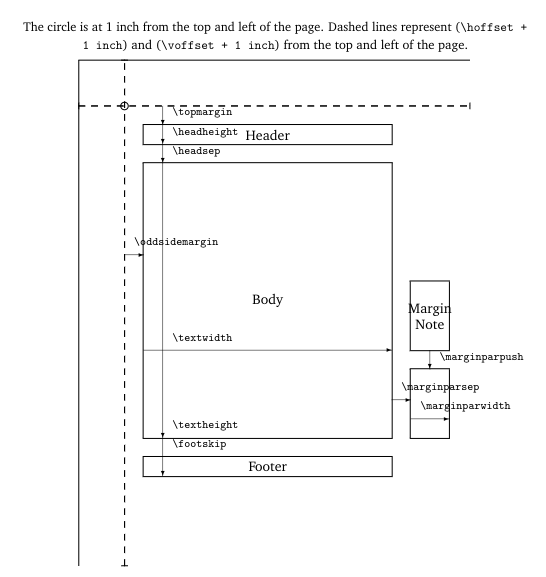
\includegraphics[width=\textwidth]{graphlet-thesis/images/layout.png}
    \caption{Dimensións das marxes utilizadas neste documento}
    \label{fig:layout}
\end{figure}

\paragraph{Tamaño do papel e marxes:} Utilizaráse un tamaño de papel A4, cos valores recomendadas para as marxes mostrados a continuación (véxase a figura \ref{fig:layout}).

\begin{center}
\begin{tabular}{ l l }
\textbackslash paperheight= 845.04694pt & \textbackslash paperwidth= 597.50793pt \\ 
\textbackslash hoffset= 0.0pt & \textbackslash voffset= 0.0pt \\
\textbackslash evensidemargin= 15.45935pt & \textbackslash oddsidemargin= 42.72656pt \\
\textbackslash topmargin= -39.24942pt & \textbackslash headheight= 17.0pt \\
\textbackslash headsep= 20.40001pt & \textbackslash textheight= 636.60028pt \\
\textbackslash textwidth= 394.78204pt & \textbackslash footskip= 185.0pt \\
\textbackslash marginparsep= 12.8401pt & \textbackslash marginparpush= 6.11995pt \\
\textbackslash columnsep= 10.0pt & \textbackslash columnseprule= 0.0pt \\
1em = 10.95pt  & 1ex = 5.2779pt \\
\end{tabular}
\end{center}
%\printinunitsof{cm}{\pagevalues}


\paragraph{Numeración das páxinas:} Tódalas páxinas deben estar numeradas, agás as que non teñan ningún contido ou a páxina de título. As páxinas non numeradas contan ingualmente. Por exemplo, a páxina de título é a  páxina (i).

As páxinas iniciais (o resumo, as dedicacións, a táboa de contidos, etc.) están numeradas con números romanos.  A partir da primeira páxina do primeiro capítulo reiníciase a numeración con números arábigos e continúa consecutivamente ata o final da tese, incluíndo os apéndices.

\paragraph{Espazo entre liñas:} Úsase interliñado simple.  Os parágrafos sepáranse por unha liña en branco (non se sangra a primeira liña do mesmo). 

\paragraph{Títulos e numeración de figuras e táboas:}  Cada táboa, figura, ilustación etc. debe ter un título indicando o elemento que pretende representar ou ilustrar.  As táboas numéranse consecutivamente ao longo do documento. As figuras, ilustracións, etc. tamén se contan consecutivamente ao longo do documento.

\paragraph{Encabezamentos e subtítulos:}     Os títulos indican a organización do documento.     Os capíutulos, secccións e subseccións débense empregar ao longo do documento, sendo coherentes no estilo e posición de cada elemento.  Cada capítulo debe comezar nunha páxina impar. 

\paragraph{Citas bibliográficas:} Débese utilizar un estilo recoñecido (tal como IEEE, APA, etc.). Recoméndase encarecidamente o uso de unha ferramenta como BibLaTeX. 


\section{Organización en seccións}
\label{sec:organización}

Este documento mostra un exemplo da posible organización dunha memoria do TFM. Descríbense a continuación as distintas seccións. 

Non existe un número de páxinas mínimo ou máximo. Non obstante, a extensión dun TFM está habitualmente entre 40 e 80 páxinas. A lonxitude variará segundo o tema elixido e o método de análise, polo que a extensión final deberá ser decidido polo autor e os seus titores. 

Unha posible organización do TFM é a seguinte (as extensións son meramente orientativas): 

\begin{enumerate}[noitemsep]
    \item Páxina de Título (obrigatorio -- 1 páxina).
    \item Resumo en inglés (\textit{abstract} -- obrigatorio -- 1 páxina).
    \item Resumo en galego ou castelán (obrigatorio -- 1 páxina).
    \item Agradecementos (opcional).
    \item Táboa de contidos (obrigatorio).
    \item Introdución (3-10 páxinas).
    \begin{enumerate}[noitemsep]
        \item Motivación.
        \item Obxectivos e presentación do problema que se vai resolver.
        \item Estrutura do documento.
    \end{enumerate}
    \item Situación actual (arpoximadamente 10-20 páxinas). Repaso do traballo relacionado, das tecnoloxías básicas, do punto de partida, etc. 
    \begin{enumerate}[noitemsep]
        \item Traballo relacionado.
        \item Tecnoloxías base.
        \item Marco de traballo (marco teórico, tecnolóxico, etc.).
    \end{enumerate}
    \item Descrición do traballo realizado (aproximadamente 10-20 páxinas). 
    \begin{enumerate}[noitemsep]
        \item Datos analizados.
        \item Análise teórica.
        \item Deseño (arquitectura, ataque, etc.).
        \item Descrición dos métodos. 
        \item Desenvolvementos realizados.
        \item Mecanismos para garantir a calidade do traballo.
    \end{enumerate}
    \item Resultados (aproximadamente 5-20 páxinas)
    \begin{enumerate}[noitemsep]
        \item Descrición dos resultados.
        \item Análise e discusión dos resultados / Validación.
    \end{enumerate}
    \item Conclusións (aproximadamente 5-10 páxinas).
    \begin{enumerate}[noitemsep]
        \item Resumo do traballo.
        \item Implicacións dos resultados / Impacto ecnonómico-social..
        \item Limitacións do traballo.
        \item Traballo futuro.
    \end{enumerate}
    \item Bibliografía (obrigatorio).
    \item Apéndices (opcional).
    \begin{enumerate}[noitemsep]
        \item Descrición de ferramentas.
        \item Descrición de configuración.
        \item Código. 
        \item Detalle adicional para algunha sección. 
        \item Etc. 
    \end{enumerate}
\end{enumerate}



\section{Obxectivos e presentación do problema}
\label{sec:intro:motivación}
{
\color{gray}
\Blindtext[3][1]

\cite{Jurgens:2000,Jurgens:1995,Miede:2011,Kohm:2011,Apple:keynote:2010,Apple:numbers:2010,Apple:pages:2010}

\cite{WEB:GNU:GPL:2010,WEB:Miede:2011}
}

\subsection{Metodoloxía}
\label{sec:intro:results:refs:method}
{
\color{gray}
\Blindtext[1][2]
}

\paragraph{Estratexia 1}
{
\color{gray}
\Blindtext[1][1]
}

\begin{lstlisting}[language=Python, caption={This simple helloworld.py file prints Hello World.}\label{lst:pyhelloworld}]
#!/usr/bin/env python
print "Hello World"
\end{lstlisting}

\paragraph{Estratexia 2}
{
\color{gray}
\Blindtext[1][1]
}

\begin{lstlisting}[language=Python, caption={This is a bubble sort function.}\label{lst:pybubblesort}]
#!/usr/bin/env python
def bubble_sort(list):
    for num in range(len(list)-1,0,-1):
        for i in range(num):
            if list[i]>list[i+1]:
                tmp = list[i]
                list[i] = list[i+1]
                list[i+1] = tmp

alist = [34,67,2,4,65,16,17,95,20,31]
bubble_sort(list)
print(list)
\end{lstlisting}

\section{Organización da memoria}
\label{sec:intro:organización}

\textbf{Capítulo \ref{sec:related}} \\[0.2em]
{
\color{gray}
\blindtext
}

\textbf{Capítulo \ref{sec:system}} \\[0.2em]
{
\color{gray}
\blindtext
}


\textbf{Capítulo \ref{sec:results}} \\[0.2em]
{
\color{gray}
\blindtext
}

\textbf{Capítulo \ref{sec:results}} \\[0.2em]
{
\color{gray}
\blindtext
}

\textbf{Capítulo \ref{sec:conclusion}} \\[0.2em]
{
\color{gray}
\blindtext
}   % INCLUDE: introduction

\chapter{Antecedentes} % SOTA
\label{sec:related}

%\cleanchapterquote{A picture is worth a thousand words. An interface is worth a thousand pictures.}{Ben Shneiderman}{(Professor for Computer Science)}

%\begin{lstlisting}[language=Java, caption={A simple Hellow World example in %Java.}\label{lst:javahelloworld}]
%public class HelloWorld {
%	public static void main ( String[] args ) {
%		// Output Hello World!
%		System.out.println( "Hello World!" );
%	}
%}
%\end{lstlisting}

A continuación veremos los elementos esenciales de esta Tesis, es importante conocer la dificultad del problema para entender la relevancia del mismo. Los elementos claves se presentan en esta sección sin embargo existe un apéndice que ayude a comprender algunos términos que podrían ayudar al lector.


\section{Redes}

Una red es un conjunto de nodos unidos por aristas que representan relaciones. Los nodos y aristas los podemos encontrar en distintas disciplinas con distintos nombres, por ejemplo en física se denominan sitios y vínculos y en sociología actores y vínculos. 

La representación matemática de un red se denomina grafo y es estudiada en matemáticas discretas y más específicamente en teoría de grafos. Un grafo esta formalmente definido como $G = (V,E)$, donde $V$ es un conjunto de nodos (vertices) y $E$ aristas (edges). \cite{saoub_graph_2021}

 \begin{figure}[htbp]
   \centering
   \includesvg[width=0.2\textwidth]{figures/graph.svg}
    \caption{Graph}
    \label{fig:graph}
\end{figure}

Un grafo dirigido o dígrafo es un grafo en el que las aristas tienen sentidos. En el sentido más formal $G = (V,E,\phi)$ donde $\phi$ es una función de incidencia que asigna cada arista a un par ordenado de nodos. $ \phi :E \to \{(x,y)\mid (x,y)\in V^{2}\ \textrm{and } x \neq y \}$

 \begin{figure}[htbp]
   \centering
   \includesvg[width=0.2\textwidth]{figures/digraph.svg}
    \caption{Directed Graph (DiGraph)}
    \label{fig:graph}
\end{figure}

Un subgrafo de un grafo $G$ es otro grafo formado a partir de un subconjunto de nodos y aristas de $G$. El subconjunto de nodos debe incluir todos los extremos del subconjunto de aristas, pero también puede incluir nodos adicionales. Un subgrafo inducido es aquel que incluye todas las aristas cuyos puntos extremos pertenecen al subconjunto de nodos.

Un isomorfismo de grafos es una biyección de los nodos de un grafo sobre otro, de modo que se preserva la adyacencia de los nodos. Formalmente, el isomorfismo entre dos grafos $G$ y $H$ se define de la siguiente manera $f:V(G) \rightarrow V(H)$ donde $f$ preserva la relación de adyacencia.

 \begin{figure}[htbp]
   \centering
   \includesvg[width=0.8\textwidth]{figures/isomorphism.svg}
    \caption{Ejemplo de Isomorfismo entre $G$ y $H$}
    \label{fig:graph}
\end{figure}

Determinar si dos grafos con el mismo número de vértices $n$ y aristas $m$ son isomorfos o no, se conoce como el problema del isomorfismo de grafos. Se trata un problema no resuelto en computación y se considera un problema NP ya que no hay prueba de que sea NP-Completo. \cite{kobler_graph_1993} [Ver Apéndice] Este problema es un caso especial del problema de isomorfismo de subgrafos que esta probado es un problema NP-Completo. Resolver el problema de isomorphismo de grafos requeriría probar si las $n!$ biyecciones posibles preservan la adyacencia, sin embargo hasta ahora no se conoce un algoritmo general para resolver el problema. 


\section{Aprendizaje de Máquina}

El Aprendizaje de Máquina, en inglés Machine Learning (ML), es una rama de la Inteligencia Artificial que estudia algoritmos y técnicas que permitan automatizar soluciones a problemas complejos a partir del aprendizaje sobre conjuntos de datos en vez de los métodos convencionales de programación. 

A diferencia de la Inteligencia Artificial, que es un campo de estudio muy amplio y utiliza distintas técnicas para crear algoritmos inteligentes, el Aprendizaje de Máquina se centra principalmente en imitar el aprendizaje humano y gradualmente mejorar la precisión sobre una tarea. \cite{ibm_what_nodate} En la programación convencional dados ciertos requerimientos se diseña un programa que siga una serie de pasos para resolver un problema. No obstante en problemas complejos, a pesar tener requerimientos claros y específicos, este enfoque puede resultar complicado crear y programar un enorme conjunto de reglas para cumplir con la tarea, pensemos por ejemplo, en la tarea de detectar objetos en una imagen. \cite{rebala_introduction_2019}

Los algoritmos de Aprendizaje de Máquina son capaces de resolver problemas de una manera un tanto más genérica aprendiendo estructuras y reglas a partir de un conjunto de datos en vez de tener una estructura y diseño explicito. Por esta razón este tipo de algoritmos dependen directamente de la calidad y cantidad de ejemplos en el conjunto de datos. Estos ejemplos pueden tener etiquetas o ser datos crudos y dependiendo de la naturaleza del conjunto de datos encontraremos distintas categorías de algoritmos dentro del Aprendizaje de Máquina. \cite{rebala_introduction_2019}

Un conjunto de datos etiquetado es aquel cuyos ejemplos tienen la respuesta a la pregunta que se hace. Puede ser una etiqueta predeterminada sobre la clase que representan, por ejemplo, una imagen de un perro que contenga la etiqueta perro. Por otro lado los datos no etiquetados (crudos) son aquellas que no contienen la respuesta correcta a la pregunta en cuestión y que deben ser explorados. 

\subsection{Aprendizaje Supervisado}

El objetivo del Aprendizaje Supervisado es crear un modelo (una serie de reglas) sobre un conjunto de datos etiquetados para posteriormente poder predecir las etiquetas de datos que no se encuentran en el conjunto de datos. \cite{rebala_introduction_2019} En esta tarea los datos tienen una etiqueta predeterminada sobre la clase que  representan, por ejemplo, una imagen de un perro que contenga la etiqueta perro. 

Esta es la manera en la que estos algoritmos resuelven problemas, primero generan un modelo aprendiendo (con un entrenamiento) sobre un conjunto de datos con etiquetas conocidas y después ejecutando el modelo aprendido para predecir la etiqueta de datos nuevos, es decir que no se encontraban en el conjunto de datos de entrenamiento. Estos algoritmos tienden a ser mas efectivos que los modelos creados por humanos ya que pueden considerar mas atributos sobre un ejemplo y pueden procesar una cantidad superior de datos. \cite{rebala_introduction_2019}

Una de las tareas principales dentro del Aprendizaje Supervisado es la Clasificación, es decir, a partir de grupos previamente predeterminados hay que identificar el grupo al que pertenece un objeto dado.

\subsection{Aprendizaje No Supervisado}

En el Aprendizaje no Supervisado la tarea principal es aprender patrones a partir de conjuntos de datos no etiquetados. En el aprendizaje no supervisado la finalidad radica en descubrir propiedades útiles de los datos disponibles.

\paragraph{Agrupamientos}

La tarea quizás mas representativa de Aprendizaje No Supervisado es el \textit{Clustering} o Agrupamiento, se trata de dividir un gran conjunto de datos (puntos) de tal manera en que los puntos con propiedades o patrones en común se encuentren en un mismo grupo. La complejidad de esta tarea radica en que los grupos no se conocen previamente y la cantidad de los mismos es desconocida. Posteriormente lo resultados de esta tarea pueden ser utilizados como clasificadores o predictores de valores de atributos desconocidos, e incluso como herramientas de visualización. \cite{kubat_introduction_2017}

 \begin{figure}[htbp]
   \centering
   \includesvg[width=0.5\textwidth]{figures/cluster-example.svg}
    \caption{Un ejemplo de Clustering en $R^2$}
    \label{fig:clustering-example}
\end{figure}

Un ejemplo sencillo de agrupamiento en $R^2$ puede ser el de la Fig. \ref{fig:clustering-example}. Aquí cada punto representa un ejemplo descrito por dos atributos. En este caso es sencillo encontrar los agrupamientos a simple vista (ojímetro), sin embargo para cuatro dimensiones o mas, no es posible para los humanos visualizar los datos ni los grupos; estos casos solo pueden ser resueltos para los algoritmos de agrupamiento. \cite{kubat_introduction_2017}

Los algoritmos de agrupamiento frecuentemente requieren definir una función de distancia entre un ejemplo y el grupo. Dependiendo de la naturaleza de los atributos distintas medidas pueden ser propuestas; cuando se trata de puntos numéricos en el espacio comúnmente se utiliza la distancia Minkowski. $X = (x_1,x_2,\ldots,x_n)$ y $Y=(y_1,y_2,\ldots ,y_n) \in R^n$
 
$$D(X,Y) = (\sum_{i=1}^{n}|x_{i}-y_{i}|^{p})^{\frac{1}{p}}$$

Quizás uno de los algoritmos más conocidos de Agrupamiento es \textit{K-Means}. Este algoritmo agrupa los datos de entrada en $K$ grupos para una $K$ predefinida por el usuario. Como cada ejemplo no incluye una etiqueta de la clase o grupo al que pertenece se trata inherentemente de un algoritmo de Aprendizaje No Supervisado. La representación matemática de de los $K$ grupos se conoce como\textit{Centroide} Un centroide es el punto promedio de la distancia a cada punto del grupo que representa. La interpretación de cada grupo, representado por su centroide, puede ser que su valor promedio es la caracterización de todos los elementos del grupo.

 \begin{figure}[htbp]
   \centering
   \includesvg[width=0.8\textwidth]{figures/centroids-example.svg}
    \caption{Centroides}
    \label{fig:cengroides}
\end{figure}

Por lo tanto, el algoritmo de \textit{K-Means} busca minimzar la distancia promedio de cada Centroide a los puntos de su grupo. Los Centroides pueden ser inicializados de manera aleatoria o con algunas técnicas de inicialización que permitan al algoritmo converger más rápido. El algoritmo se itera recalculado los centroides y los puntos correspondientes hasta que ya no hay un cambio significativo o se ejecuta el número máximo de interaciones. Uno de los aspectos negativos de este algoritmo es que es muy susceptible a las condiciones iniciales y por lo tanto se recomienda ejecutar el algoritmo varias veces.

\lstinputlisting[language=Python, caption={Pseudocódigo $K-Means$ \cite{kubat_introduction_2017}}\label{algorithms:k-means}]{codes/kmeans.pseudo} 

\section{Métodos para agrupar redes}

\subsection{Embeddings}

\subsection{Propiedades de la Red}
\label{sec:related:sec2}

\subsection{Propiedades de los Nodos}
\label{sec:related:sec2}

\section{Interpretabilidad}
\label{sec:related:sec3}

A pesar de que los algoritmos de Aprendizaje de Máquina funcionan muy bien, muchas veces es difícil conocer las reglas que el algoritmo ha creado en el modelo aprendido y por lo tanto no es posible comprender como es que un problema esta siendo resuelto, a este problema se le conoce como el problema de interpretabilidad de un modelo. \cite{rebala_introduction_2019} 

Este problema esta especialmente presente en las Redes Neuronales que tienen millones de parámetros y por lo tanto es complicado interpretar las decisiones o la serie de reglas que llevan a cabo para resolver un problema. En algunas áreas es igual de importante la interpretabilidad del modelo que su precisión, un ejemplo claro es el de la medicina en donde los médicos deben ser capaces de interpretar y confirmar los resultados del diagnóstico de un algoritmo.

En el contexto de Twitter es igualmente importante interpretar los motivos por los que las redes son agrupadas.

Explicar que en el contexto de Twitter nos importa no sólo cómo quedan los grupos sino por qué. 
Redes sociales, lo que sociólogos han hecho con estas ideas
(como en la parte de antecedentes del paper)   % INCLUDE: state of the art

%\part{Exemplo doutra parte}
% !TEX root = ../my-thesis.tex
%
\chapter{Propuesta}
\label{sec:system}

\cleanchapterquote{Innovation distinguishes between a leader and a follower.}{Steve Jobs}{(CEO Apple Inc.)}


{
\color{gray}
\Blindtext[2][1]
}

\section{Arquitectura dos desenvolvementos}
\label{sec:system:sec1}
{
\color{gray}
\Blindtext[1][2]
}

\begin{figure}[htb]
	
\includegraphics[width=\textwidth]{images/Clean-Thesis-Figure}
	\caption{Figure example: \textit{(a)} example part one, \textit{(c)} example part two; \textit{(c)} example part three}
	\label{fig:system:example1}
\end{figure}

{
\color{gray}
\Blindtext[1][2]
}

\section{Datos}
\label{sec:system:sec2}

{
\color{gray}
\Blindtext[1][2]
}

\begin{figure}[htb]
	
\includegraphics[width=\textwidth]{images/Clean-Thesis-Figure}
	\caption{Another Figure example: \textit{(a)} example part one, \textit{(c)} example part two; \textit{(c)} example part three}
	\label{fig:system:example2}
\end{figure}

{
\color{gray}
\Blindtext[2][2]
}

\section{Análise teórica}
\label{sec:system:sec3}
{
\color{gray}
\Blindtext[4][2]
}

\section{Deseño}
\label{sec:system:design}
{
\color{gray}
\Blindtext[2][1]
}         % INCLUDE: proposal

\chapter{Experimentos y Resultados}
\label{sec:results}

\cleanchapterquote{Users do not care about what is inside the box, as long as the box does what they need done.}{Jef Raskin}{about Human Computer Interfaces}
\section{Dataset}
\label{sec:concepts:sec1}
{
\color{gray}
\Blindtext[2][2]
}

{
\color{gray}
\Blindtext[2][1]
}


\section{Experimentos}
\label{sec:concepts:sec1}
{
\color{gray}
\Blindtext[2][2]
}

\subsection{Conteos}
\label{sec:intro:results:refs:method}
{
\color{gray}
\Blindtext[1][2]
}

\section{Resultados}
\label{sec:concepts:sec2}
{
\color{gray}
\Blindtext[3][2]
}

\subsection{Visualización}
\label{sec:intro:results:refs:method}
{
\color{gray}
\Blindtext[1][2]
}

\section{Discusión}
\label{sec:concepts:sec3}
{
\color{gray}
\Blindtext[3][2]
}

\subsection{Perfiles encontrados}
\label{sec:intro:results:refs:method}
{
\color{gray}
\Blindtext[1][2]
}

       % INCLUDE: concepts

\chapter{Conclusiones}
\label{sec:conclusion}

{
\color{gray}
\Blindtext[2][1]
}
\section{Resumen}
\label{sec:conclusion:sec1}
{
\color{gray}
\Blindtext[2][2]
}

\section{Implicaciones}
\label{sec:conclusion:sec2}
{
\color{gray}
\Blindtext[3][2]
}

\section{Limitaciones y trabajo futuro}
\label{sec:conclusion:future}
{
\color{gray}
\Blindtext[2][2]
}     % INCLUDE: conclusion

% --------------------------
% Back matter
% --------------------------
%

%\cleardoublepage

%\listoffigures
%\cleardoublepage

%\listoftables
%\cleardoublepage

%\lstlistoflistings
%\cleardoublepage

\appendix\cleardoublepage

\chapter{Apéndice}
\label{sec:appendix}

{
\color{gray}
\Blindtext[1][1]
}

\section{Capítulo 2}
\label{sec:appendix:sec2}

\paragraph{Función Biyectiva}

Una función es biyectiva es aquella que es a la vez inyectiva y suprayectiva. Es decir, una función entre los elementos de dos conjuntos, donde cada elemento de un conjunto se empareja con exactamente un elemento del otro conjunto, y cada elemento del otro conjunto se empareja con exactamente un elemento del primer conjunto.

Formalmente, dada una función $f$

$ {\begin{array}{rccl}f:&X&\longrightarrow &Y\\&x&\longmapsto &y=f(x)\end{array}} $

Es biyectiva si para todo $y$ de $Y$ existe un único $x$ de $X$ al que la función evaluada en $x$ es igual a $y$

$ \forall y\in Y\;:\quad \exists !\ x\in X\;/\quad f(x)=y $

\paragraph{Problema NP}



\section{Sección 2}
\label{sec:appendix:sec2}


{
\color{gray}
\Blindtext[1][1]

\begin{table}[h]
	\begin{tabularx}{\textwidth}{X | X | X}
		%\hline
		Alpha		& Beta			& Gamma			\\ \hline
		0			& 1				& 2				\\ \hline
		3			& 4				& 5				\\ %\hline
	\end{tabularx}
	\label{tab:table2}
	\caption{This is a caption text.}
\end{table}


\Blindtext[1][2]
}       % INCLUDE: appendix

{%
\setstretch{1.1}
\renewcommand{\bibfont}{\normalfont\small}
\setlength{\biblabelsep}{0pt}
\setlength{\bibitemsep}{0.5\baselineskip plus 0.5\baselineskip}
\printbibliography[]
%\printbibliography[nottype=online]
%\newrefcontext[labelprefix={@}]
%\printbibliography[heading=subbibliography,title={Webpages},type=online]

}

\newpage
\mbox{}

% **************************************************
% End of Document CONTENT
% **************************************************
\end{document}
